\chapter{Tutorial}
\label{chpt:Tutorial}
\typeout{$Id$}

\section{Connecting to a database}

\begin{figure}[hpt]
\begin{centering}
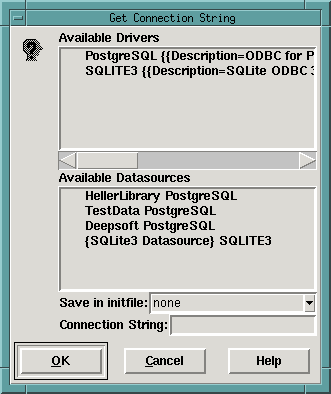
\includegraphics{GetConnectionStringDialog.png}
\caption{Get Connection String Dialog box}
\label{fig:tut:getconnectionstring}
\end{centering}
\end{figure}
\begin{figure}[hpt]
\begin{centering}
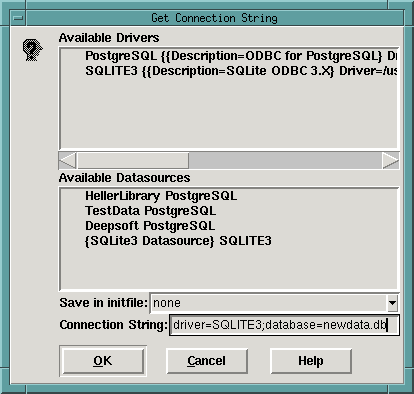
\includegraphics{GetConnectionStringDialogSQLite.png}
\caption{Get Connection String Dialog box, with connection string filled in}
\label{fig:tut:getconnectionstringsqlite}
\end{centering}
\end{figure}
The Home Librarian uses a database ``back end'' to store the card
records. It is possible to use one of several different database
systems, including PostgreSQL, MySQL, Sqlite, SQL Server, and others.
All you need is a ODBC driver library installed. The Home Librarian
attempts to connect to a database on startup.  It reads in one of a set
of configuration files for a connection string.  If it does not find
either the configuration files or if there isn't a valid connection
string in these files, it will prompt for a connection string using a
``Get Connection String Dialog'' (described in
Section~\ref{sect:ref:getconnectionstring}). A typical ``Get Connection
String Dialog'' box is shown in
Figure~\ref{fig:tut:getconnectionstring}. In
Figure~\ref{fig:tut:getconnectionstringsqlite} is a ``Get Connection
String Dialog'' with a connection string filled in.  Selecting ``OK''
will connect to the database.

\begin{figure}[hpt]
\begin{centering}
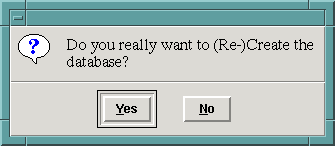
\includegraphics{ReCreateDB.png}
\caption{(Re-)Create the database question box}
\label{fig:tut:recreatedatabase}
\end{centering}
\end{figure}
When you connect to a new database or a database never before used with
the Home Librarian program, a dialog box prompting confirmation to
(re-)create the database is displayed, as shown in
Figure~\ref{fig:tut:recreatedatabase}. 

\begin{figure}[hpt]
\begin{centering}
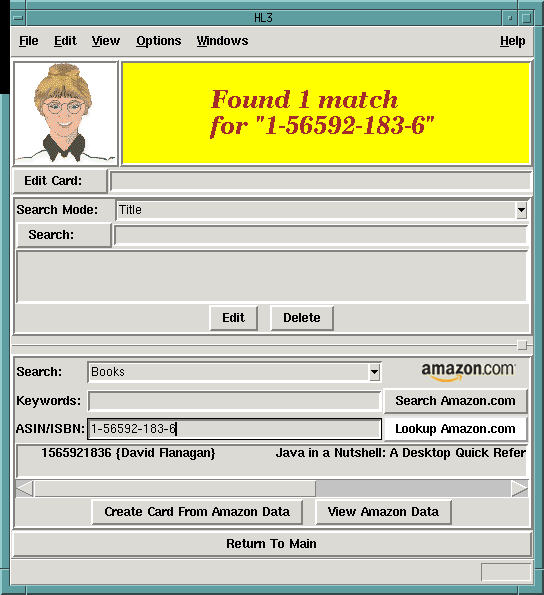
\includegraphics[width=5in]{AmazonSearchJavaNutshell.png}
\caption{Amazon search results for 1-56592-183-6}
\label{fig:tut:Amazonsearchjavanut}
\end{centering}
\end{figure}
\begin{figure}[hpt]
\begin{centering}
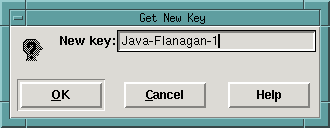
\includegraphics{EnterNewKey.png}
\caption{Entering a new key}
\label{fig:tut:newkeyjava1}
\end{centering}
\end{figure}
\begin{figure}[hpt]
\begin{centering}
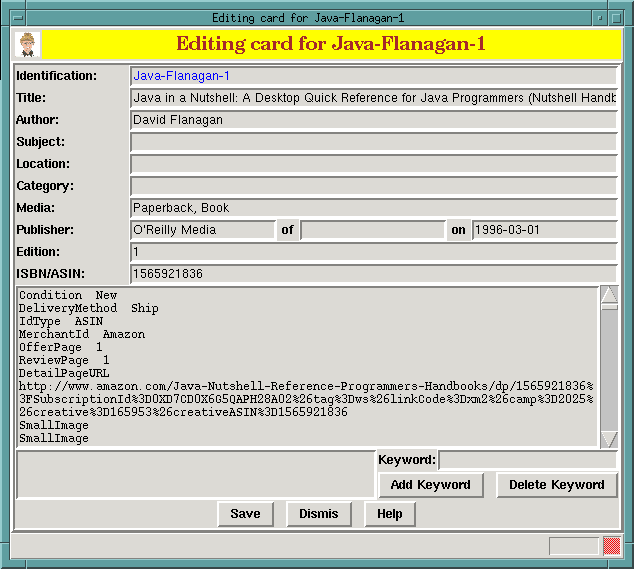
\includegraphics[width=5in]{Java-Flanagan-1-Initial.png}
\caption{Initialized card for Java in a Nutshell}
\label{fig:tut:javaflanagan1initial}
\end{centering}
\end{figure}
\begin{figure}[hpt]
\begin{centering}
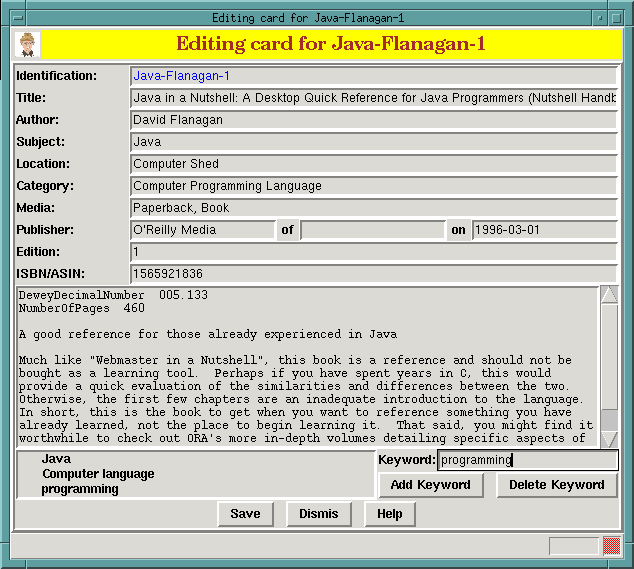
\includegraphics[width=5in]{Java-Flanagan-1-Edited.png}
\caption{edited card for Java in a Nutshell}
\label{fig:tut:javaflanagan1editedl}
\end{centering}
\end{figure}
Once connected to a database, it is now possible to add cards to the
database, using the ``Update Library'' function. One way to add cards
is to search on Amazon for information about items in your library. For
example if the book ``Java in a Nutshell'' with ISBN number
1-56592-183-6, you can perform the search shown in
Figure~\ref{fig:tut:Amazonsearchjavanut}. We can now hightlight the
search result and create a card from it.  We are prompted for a new key
to uniquely identify this item, as shown in
Figure~\ref{fig:tut:newkeyjava1}. We now have a new card record with
most of its fields filled out from the Amazon data, shown in
Figure~\ref{fig:tut:javaflanagan1initial}.  After a bit of editing, the
card editor looks like Figure~\ref{fig:tut:javaflanagan1edited}.  The
Subject, Location, and Category fields have been filled in.  The
Descriptive text has been trimmed, and a collection of keywords added.

We can now save this card in the database by clicking on the ``Save''
button. We now have a database with this card in it.  We can now perform
some searches using the search screen.

\begin{figure}[hpt]
\begin{centering}
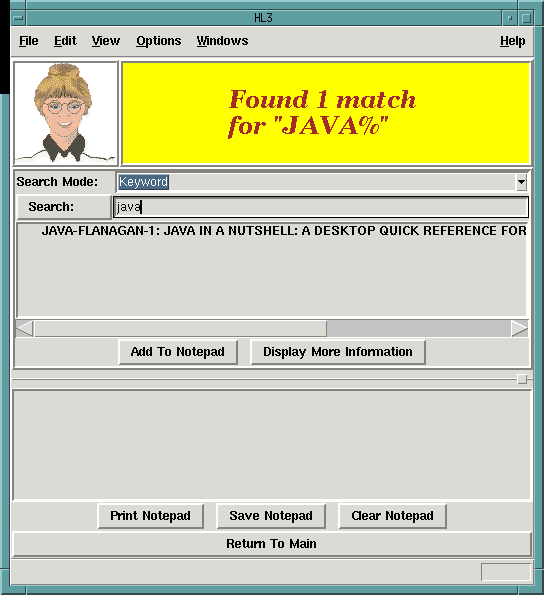
\includegraphics[width=5in]{SearchKeywordJava.png}
\caption{Searching for keyword ``java''}
\label{fig:tut:searchkeywordjava}
\end{centering}
\end{figure}
\begin{figure}[hpt]
\begin{centering}
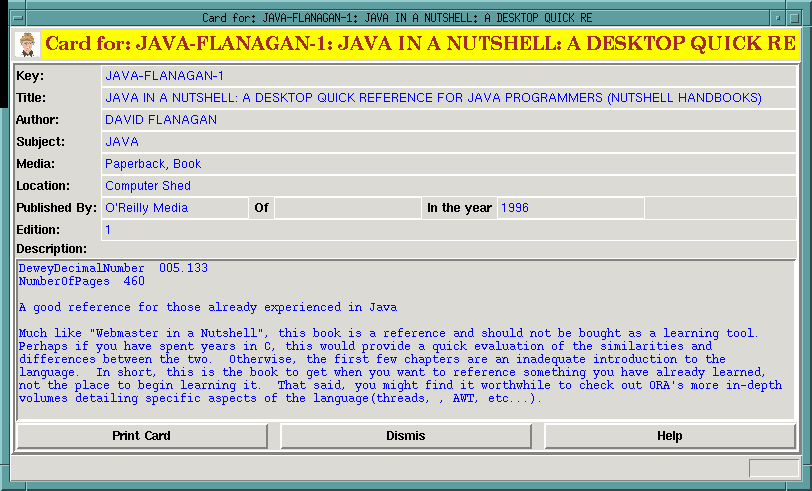
\includegraphics[width=5in]{MoreInformationJavaFlanagan1.png}
\caption{More information about Java-Flanagan-1}
\label{fig:tut:moreinfojavaflanagan1}
\end{centering}
\end{figure}
A card database can be searched in several ways. 
Figure~\ref{fig:tut:searchkeywordjava} shows a search by keyword using
the keyword ``java''. And Figure~\ref{fig:tut:moreinfojavaflanagan1}
shows what is displayed when the search result is highlighted and the
``Display More Information'' button is clicked.

